\documentclass[10pt]{beamer}
\usepackage[slovene]{babel}
\usepackage[utf8]{inputenc}
\usepackage[T1]{fontenc}
\usepackage{lmodern}
\usepackage{mathptmx}
\usepackage{helvet}
\usepackage{courier}
\usepackage{hyperref}
\usepackage{wrapfig}
\usepackage{tikz}
\usepackage{tcolorbox}

\usetheme{CambridgeUS}

\begin{document}

\title[Finančni instrumenti osnovani na razpršenosti]{Finančni instrumenti osnovani na razpršenosti}
\author{Žan Jarc}
\institute [FMF]{ Fakulteta za matematiko in fiziko}

\begin{frame}
	\titlepage
\end {frame}

\begin{frame}
\textbf{Vsebina predstavitve}:
	\begin{itemize}
		\item Volatilnost trga
		\item Standard \& Poor’s 500 indeks
		\item VIX
		\item VIX terminski posli (futures) in VIX opcije (options)
			\begin{itemize}
				\item VIX terminski posli
				\item VIX opcije
			\end{itemize}
	\end{itemize}
\end {frame}

\begin{frame}
\frametitle{Volatilnost trga}
\begin{itemize}
\item \textbf{Volatilnost trga} je volatilnost donosov finančnih instrumentov/naložb.

\item Volatilnost nam implicira razlike donosov.

\item Če se trg strmo dviga/pada bo volatilnost visoka.
\item Govorimo lahko o trenutni volatilnosti (actual volatility) ali o prihodnji volatilnosti (implied volatility).
\end{itemize}
\end{frame}

\begin{frame}
\frametitle{Standard \& Poor’s 500 indeks}
\begin{itemize}
\item \textbf{Standard \& Poor’s 500} ali \textbf{S\&P 500} indeks je najbolj uporabljena referenčna meritev za splošen ameriški delniški trg.
\item Je kapitalizacijsko otežen indeks. 
\item Pri računanju indeska se upošteva cene delnic 500 največjih ameriških podjetij in število delnic posamenznega podjetja, ki so na voljo na odprtem trgu.
\item Ticker SPX

\end{itemize}
\end{frame}

\begin{frame}
\frametitle{SPX med letoma 2004 in 2019}
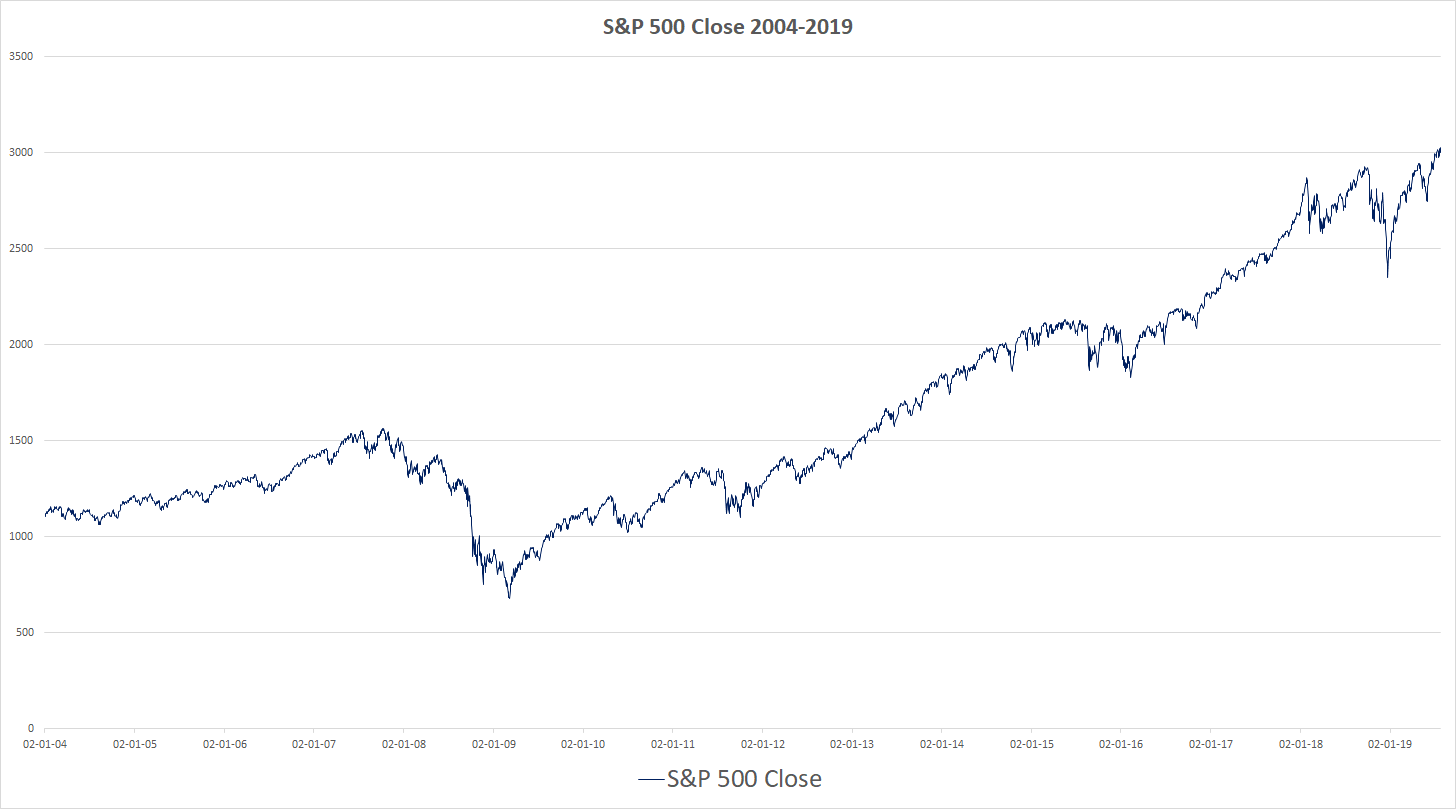
\includegraphics[width=1\textwidth]{./Grafi/SPX 2004-2019.png}
\end{frame}

\begin{frame}
\frametitle{SPX 2019}
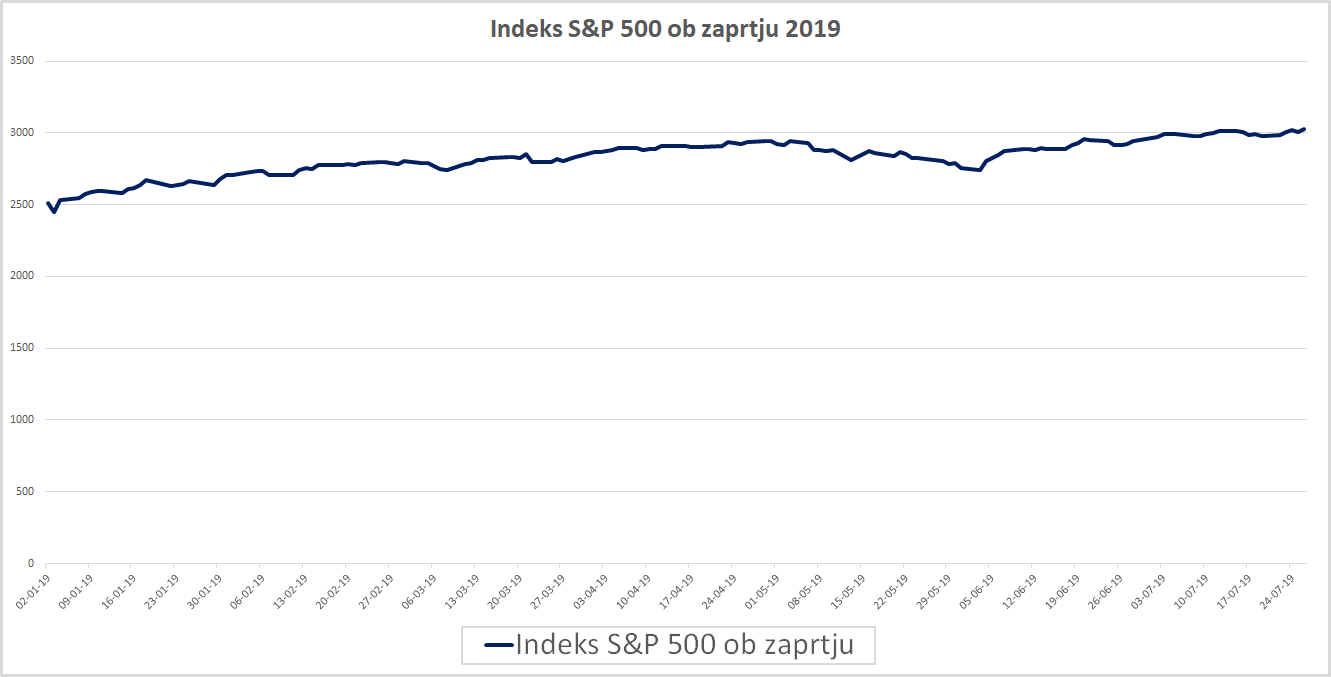
\includegraphics[width=1\textwidth]{./Grafi/SPX 2019.png}
\end{frame}

\begin{frame}
\frametitle{Volatility Index}
\begin{itemize}
\item \textbf{Cboe Volatility Index} ali \textbf{VIX} je bil razvit za napovedovanje pričakovane volatilnosti.
\item Indeks prikazuje 30 dnevno pričakovano volatilnost vseh out-of-the-money S\&P 500 nakupnih in prodajnih opcij, ki se iztečejo čez več kot 23 in manj kot 37 dni. 
\item Odraža pričakovanje trga, kako bo trg nihal v prihodnjih 30 dneh.
\item Omenja se ga tudi pod imenom "Fear Index"
\end{itemize}
\end{frame}

\begin{frame}
\frametitle{VIX in SPX primerjava}
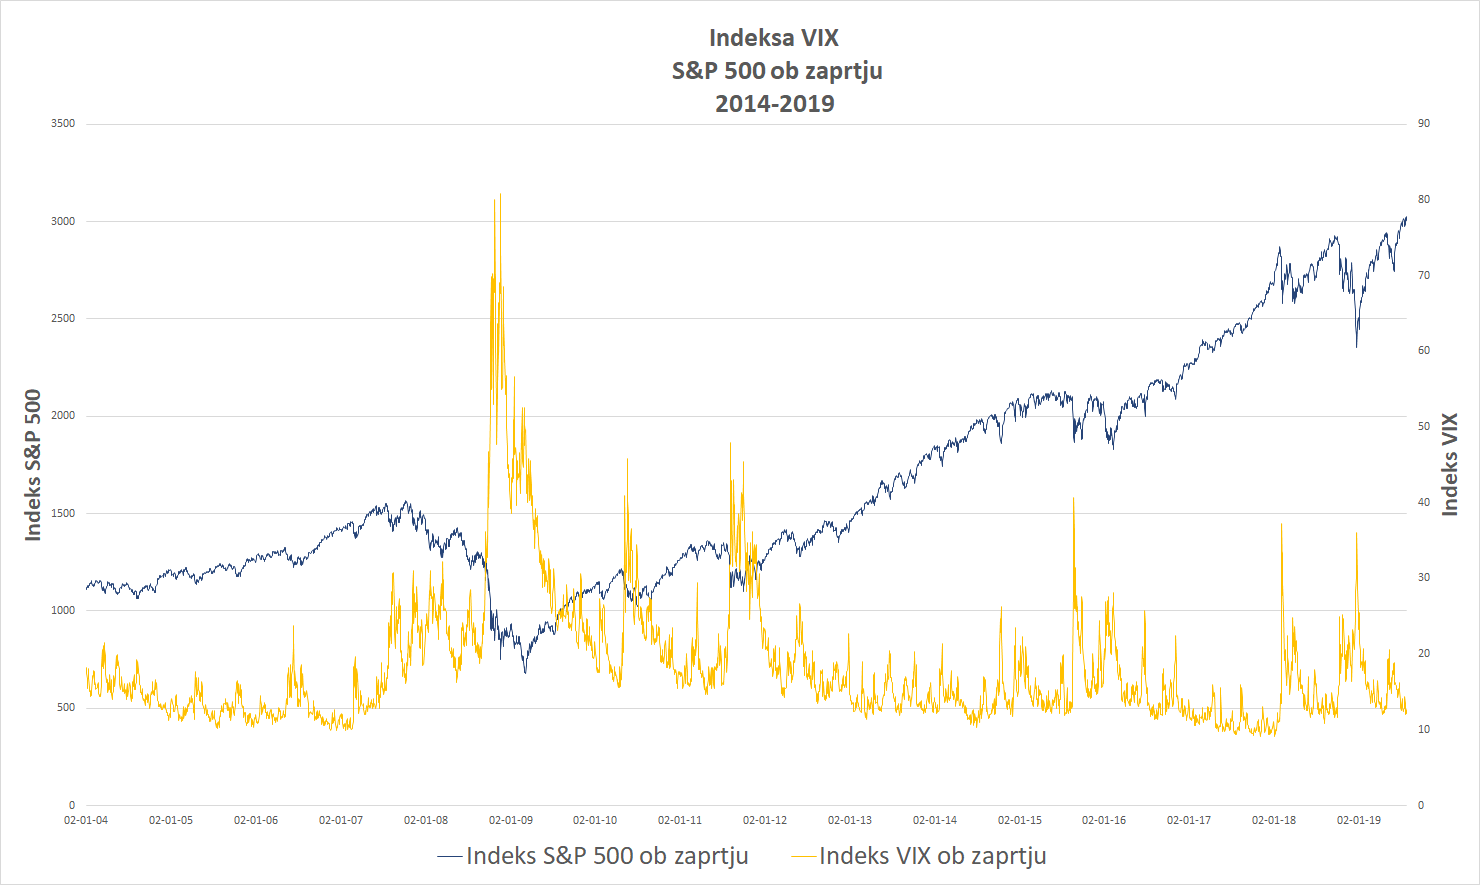
\includegraphics[width=1\textwidth]{./Grafi/VIX vs SPX 2004-2019.png}
\end{frame}

\begin{frame}
\frametitle{Lastnosti VIX}
\begin{itemize}
\item VIX in SPX sta povezana z negativno korelacijo.
\item Negativna korelacija je najbolj izrazita ko finančni trgi doživijo velike izgube npr. za čas finančne krize med letoma 2008 in 2009. 
\item SPX je oktobra 2007 dosegel 1565,15 točk, najnižjo vrednost pa je dosegel marca 2009, ko je bila vrednosti 676,53. 
\item V istem časovnem okvirju je VIX zrasel iz 16,12 na 49,68 točke (vrh je dosegel novembra 2008 z vrednostjo 80,86). 
\item Ker je VIX le merilo volatilnosti trga, z njim ne moremo investirati.
\item Zato obstajajo različni finančni inštrumenti, s katerimi lahko pridobimo izpostavljenost proti VIX indeksu, VIX terminski posli in VIX opcije.
\end{itemize}
\end{frame}

\begin{frame}
\frametitle{VIX terminski posli}
\begin{itemize}
\item VIX terminski posli so v uporabi že od leta 2004 in jih najdemo pod kratico VX in VX01 do VX53.
\item Terminski posli se iztečejo na sredo, ki je 30 dni pred petkom, ko se iztečejo SPX opcije.
\item Vrednost terminskega posla s časom konvergira k vrednosti VIX. Zaradi tega so terminski posli, ki se bodo kmalu iztekli veliko bolj občutljivi na spremembe VIX, kot pa tisti z daljšo ročnostjo. Posli z daljšo ročnostjo imajo tudi višjo premijo.
\item Če investiramo v terminski posel z dolge pozicije, ko je VIX nizek, pričakujemo, da se bo volatilnost trga povišala, drugače bomo na izgubi (contango). 
\item Ob primeru, da je volatilnost trga visoka, pa z nakupom dolge pozicije terminskega posla menimo, da se bo volatilnost zmanjšala (backwardation). 
\end{itemize}
\end{frame}

\begin{frame}
\frametitle{VIX terminski posli 2018}
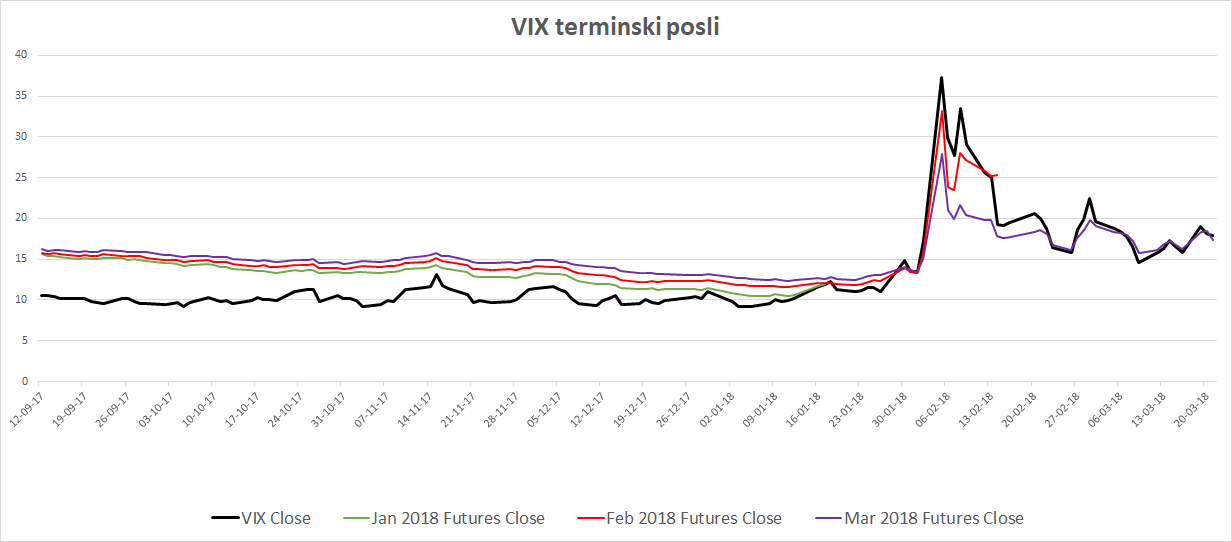
\includegraphics[width=1\textwidth]{./Grafi/VIX futures 2018.png}
\end{frame}










\begin{frame}
\frametitle{Viri}
	\begin{itemize}
		\item
			\label{Pickety}
			T.~Pickety, \emph{Capital in the twenty-first century}, The Belknap Press of 						Harvard University Press, London, 2014.

		\item 
			\label{Razdelitev premoženja}
			\emph{Distribution of wealth}, v: Wikipedia, The Free Encyclopedia, [ogled 							20.~4.~2019], dostopno na \url{https://en.wikipedia.org/w/index.php?								title=Distribution_of_wealth&oldid=854198883}.

		\item 
			\label{Metrike ekonomske neenakosti}
			\emph{Income inequality metrics}, v: Wikipedia, The Free Encyclopedia, [ogled 					20.~4.~2019], dostopno na \url{https://en.wikipedia.org/w/index.php?								title=Income_inequality_metrics&oldid=853906711}.

\item
\emph{Ginijev koeficient}, Janja Trogar, [ogled 3.~5.~2019], dostopno na \url{https://repozitorij.uni-lj.si/IzpisGradiva.php?id=97164}.

\item
\emph{Statistični urad RS}, Neenakost porazdelitve dohodka - Ginijev količnik (\%), Slovenija, letno, [ogled 4.~5.~2019], dostopno na \url{https://pxweb.stat.si/pxweb/Dialog/varval.asp?ma=0867312S&ti=&path=../Database/Dem_soc/08_zivljenjska_raven/08_silc_kazalniki_revsc/15_08673_porazdel_dohodka/&lang=2}.


\end{itemize}
\end {frame}

\begin{frame}
\frametitle{Viri}
\begin{itemize}
\item
F.~Solt, \emph{Economic Inequality and Democratic Politcal Engagement}, American Journal of Political Science, Southern Illinois University, 2008.		
\item{Svetovna banka},[ogled 22.4.2019], dostopno na \url{https://data.worldbank.org/topic/poverty}	
	

\end{itemize}
\end{frame}










\end{document}